%% ---
%% INICIO DAS CUSTOMIZACOES PARA A UNIVERSIDADE TECNOLÓGICA FEDERAL DO PARANÁ - CAMPUS PATO BRANCO
%% AUTOR: IGOR SANTANA SOUSA - 2017
%% ---

\documentclass[
% -- opções da classe memoir --
	12pt,				  % tamanho da fonte
	openright,		% capítulos começam em pág ímpar (insere página vazia caso preciso)
	twoside,			% para impressão em recto e verso. Oposto a oneside
	a4paper,			% tamanho do papel.
% -- opções da classe abntex2 --
	chapter=TITLE,		    % títulos de capítulos convertidos em letras maiúsculas
	% section=TITLE,		    % títulos de seções convertidos em letras maiúsculas
	%subsection=Title,	  % títulos de subseções convertidos em letras maiúsculas
	%subsubsection=TITLE, % títulos de subsubseções convertidos em letras maiúsculas
% -- opções do pacote babel --
	english,			% idioma adicional para hifenização
%	french,				% idioma adicional para hifenização
%	spanish,			% idioma adicional para hifenização
	brazil				% o último idioma é o principal do documento
	]{abntex2}

% ---
% Pacotes básicos
% ---
\usepackage{lmodern}			  % Usa a fonte Latin Modern
\usepackage[T1]{fontenc}		% Selecao de codigos de fonte.
\usepackage[utf8]{inputenc}	% Codificacao do documento (conversão automática dos acentos)
\usepackage{lastpage}			  % Usado pela Ficha catalográfica
\usepackage{indentfirst}		% Indenta o primeiro parágrafo de cada seção.
\usepackage{color}				  % Controle das cores
\usepackage{graphicx}			  % Inclusão de gráficos
\usepackage{microtype} 			% para melhorias de justificação
% --- Packages included 
\usepackage{xfrac}
\usepackage{amsmath} % auxilia na equacoes matematicas
\usepackage{amssymb,wasysym,latexsym,amsfonts,textcomp} % insercao de simbolos
\usepackage{mathrsfs}

\usepackage{chngcntr} % numeracao de figuras e tabelas conforme os capitulos
\counterwithin{figure}{chapter}
\counterwithin{table}{chapter}

\usepackage{listings} % Inserção de código fonte
\renewcommand{\lstlistingname}{Algoritmo}% Listing -> Algorithm
\renewcommand{\lstlistlistingname}{Lista de \lstlistingname~s}% List of Listings -> List of Algorithms
% Configurações do pacote 'listings'
\lstset{%
    basicstyle=\ttfamily,columns=fullflexible,
	showspaces = false, % Marcar espaços
	showstringspaces = false, % Marcar os espaços nas strings
	showtabs = false, % Marcar tabs
	numbers = left, % Posição dos números de linha (Remova para eles desaparecerem)
	tabsize = 2, % Número de espaços por tab
	mathescape = true, % Permite o ambiente de equações
    xleftmargin = 20pt,
}
% ---
% Pacotes adicionais, usados apenas no âmbito do Modelo Canônico do abnteX2
% ---
% ---
% Pacotes de citações
% ---
% \usepackage[brazilian,hyperpageref]{backref}	  % Paginas com as citações na bibl
\usepackage[brazilian,hyperpageref]{}	  % Paginas com as citações na bibl
%\usepackage[alf]{abntex2cite}	                % Citações padrão ABNT
\usepackage[alf,abnt-emphasize=bf]{abntex2cite} % -igor | Referências configuradas para estar alinhadas a esquerda com título em negrito

% Pacote de customizações
\usepackage{customizacoes}  % -igor | Adiciona o pacote de customizações (Nota 1)

\usepackage{tikz}	% -igor | Pacote necessaŕio para incorporar o figura fundo da capa

% ---
% CONFIGURAÇÕES DE PACOTES
% ---

% ---
% Configurações do pacote backref
% Usado sem a opção hyperpageref de backref
% \renewcommand{\backrefpagesname}{Citado na(s) página(s):~}
% % Texto padrão antes do número das páginas
% \renewcommand{\backref}{}
% % Define os textos da citação
% \renewcommand*{\backrefalt}[4]{
% 	\ifcase #1 %
% 		Nenhuma citação no texto.%
% 	\or
% 		Citado na página #2.%
% 	\else
% 		Citado #1 vezes nas páginas #2.%
% 	\fi}%
% % ---

% -igor | Pacotes necessaŕios para a configuração dos quadros
\usepackage{longtable,ltcaption} % -igor | Para as tabelas
%\usepackage{floatrow}
%\floatsetup[figure]{capposition=top}

% -igor | ??
\usepackage[font=footnotesize]{caption}

% ---
% Informações de dados para CAPA e FOLHA DE ROSTO
% ---
\titulo{Verificação e Validação Numérica do Algoritimo GMRES na solução de
Problemas de Transferência de Calor utilizando Método de Diferenças Finitas}                                % -igor | Título do trabalho (Nota 2)
\autor{Paulo Adriano Gemo Conci}                                     % -igor | Nome do autor do trabalho
\local{PATO BRANCO}                                       % -igor | Local onde foi feito o trabalho
\data{2019}                                               % -igor | Ano no qual foi finalizado o trabalho (??)
\orientador{Prof.\ Dr.\ Francisco Augusto Aparecido Gomes}       % -igor | Orientador do trabalho
\coorientador{}                             % -igor | Coorientador (caso exista)
\instituicao{%
	UNIVERSIDADE TECNOLÓGICA FEDERAL DO PARANÁ\\            % -igor | Instituição (Nota 2)
	DEPARTAMENTO ACADÊMICO DE MECÂNICA\\                    % -igor | Instituição (Nota 2)
	CURSO DE ENGENHARIA MECÂNICA}                           % -igor | Instituição (Nota 2)
\tipotrabalho{TRABALHO DE CONCLUSÃO DE CURSO}             % -igor | Tipo de trabalho
% O preambulo deve conter o tipo do trabalho, o objetivo,
% o nome da instituição e a área de concentração
\preambulo{Trabalho de conclusão de curso de graduação, apresentado à
disciplina de Trabalho de Conclusão de Curso I, do Curso de Engenharia Mecânica
do Departamento Acadêmico de Mecânica~-~DAMEC~-~da Universidade Tecnológica
Federal do Paraná, como requisito parcial para obtenção do título de Bacharel
em Engenharia Mecânica.}               % -igor | Texto do preâmbulo
% ---

% ---
% Configurações de aparência do PDF final

% alterando o aspecto da cor azul
\definecolor{blue}{RGB}{41,5,195}

% informações do PDF
\makeatletter
% \usepackage[a-1b]{pdfx}
\hypersetup{%
  %pagebackref=true,
	% pdftitle={\@title},
	% pdfauthor={\@author},
  pdfsubject={\imprimirpreambulo},
	pdfcreator={LaTeX with abnTeX2},
	pdfkeywords={abnt}{latex}{abntex}{abntex2}{trabalho acadêmico},
	colorlinks=true,       		% false: boxed links; true: colored links
	linkcolor=black,          % color of internal links
	citecolor=black,        	% color of links to bibliography
	filecolor=black,      		% color of file links
	urlcolor=black,
	bookmarksdepth=4
}
\makeatother
% ---

% ---
% Espaçamentos entre linhas e parágrafos
% ---

% -igor | Configuração do tamanho do parágrafo
\setlength{\parindent}{1cm}

% Controle do espaçamento entre um parágrafo e outro:
\setlength{\parskip}{0cm}  % tente também \onelineskip

% ---
% compila o indice
% ---
\makeindex
% ---

% ----
% Início do documento
% ----
\begin{document}

% Seleciona o idioma do documento (conforme pacotes do babel)
%\selectlanguage{english}
\selectlanguage{brazil}

% Retira espaço extra obsoleto entre as frases.
\frenchspacing

% ----------------------------------------------------------
% ELEMENTOS PRÉ-TEXTUAIS
% ----------------------------------------------------------
% \pretextual

% ---
% Capa
% ---
\imprimircapa%
% ---

% ---
% Folha de rosto
% (o * indica que haverá a ficha bibliográfica)
% ---
\imprimirfolhaderosto*
% ---

% ---
% Inserir a ficha bibliografica
% ---

% Isto é um exemplo de Ficha Catalográfica, ou ``Dados internacionais de
% catalogação-na-publicação''. Você pode utilizar este modelo como referência.
% Porém, provavelmente a biblioteca da sua universidade lhe fornecerá um PDF
% com a ficha catalográfica definitiva após a defesa do trabalho. Quando estiver
% com o documento, salve-o como PDF no diretório do seu projeto e substitua todo
% o conteúdo de implementação deste arquivo pelo comando abaixo:
%
% \begin{fichacatalografica}
%     \includepdf{fig_ficha_catalografica.pdf}
% \end{fichacatalografica}

%\begin{fichacatalografica}
%	\sffamily
%	\vspace*{\fill}					% Posição vertical
%	\begin{center}					% Minipage Centralizado
%	\fbox{\begin{minipage}[c][8cm]{13.5cm}		% Largura
%	\small
%	\imprimirautor
	%Sobrenome, Nome do autor

%	\hspace{0.5cm} \imprimirtitulo  / \imprimirautor. --
%	\imprimirlocal, \imprimirdata-

%	\hspace{0.5cm} \pageref{LastPage} p. : il. (algumas color.) ; 30 cm.\\

%	\hspace{0.5cm} \imprimirorientadorRotulo~\imprimirorientador\\

%	\hspace{0.5cm}
%	\parbox[t]{\textwidth}{\imprimirtipotrabalho~--~\imprimirinstituicao,
%	\imprimirdata.}\\

%	\hspace{0.5cm}
%		1. Palavra-chave1.
%		2. Palavra-chave2.
%		2. Palavra-chave3.
%		I. Orientador.
%		II. Universidade xxx.
%		III. Faculdade de xxx.
%		IV. Título
%	\end{minipage}}
%	\end{center}
%\end{fichacatalografica}
% ---

% ---
% Inserir errata
% ---
%\begin{errata}
%Elemento opcional da \citeonline[4.2.1.2]{NBR14724:2011}. Exemplo:

%\vspace{\onelineskip}

%FERRIGNO, C. R. A. \textbf{Tratamento de neoplasias ósseas apendiculares com
%reimplantação de enxerto ósseo autólogo autoclavado associado ao plasma
%rico em plaquetas}: estudo crítico na cirurgia de preservação de membro em
%cães. 2011. 128 f. Tese (Livre-Docência) - Faculdade de Medicina Veterinária e
%Zootecnia, Universidade de São Paulo, São Paulo, 2011.

%\begin{table}[htb]
%\center
%\footnotesize
%\begin{tabular}{|p{1.4cm}|p{1cm}|p{3cm}|p{3cm}|}
%  \hline
%   \textbf{Folha} & \textbf{Linha}  & \textbf{Onde se lê}  & \textbf{Leia-se}  \\
%    \hline
%    1 & 10 & auto-conclavo & autoconclavo\\
%   \hline
%\end{tabular}
%\end{table}

%\end{errata}
% ---

% ---
% Inserir folha de aprovação
% ---

% Isto é um exemplo de Folha de aprovação, elemento obrigatório da NBR
% 14724/2011 (seção 4.2.1.3). Você pode utilizar este modelo até a aprovação
% do trabalho. Após isso, substitua todo o conteúdo deste arquivo por uma
% imagem da página assinada pela banca com o comando abaixo:
%
% \includepdf{folhadeaprovacao_final.pdf}
%
%\begin{folhadeaprovacao}

%  \begin{center}
%    {\ABNTEXchapterfont\large\imprimirautor}

%    \vspace*{\fill}\vspace*{\fill}
%    \begin{center}
%      \ABNTEXchapterfont\bfseries\Large\imprimirtitulo
%    \end{center}
%    \vspace*{\fill}

%    \hspace{.45\textwidth}
%    \begin{minipage}{.5\textwidth}
%        \imprimirpreambulo
%    \end{minipage}%
%    \vspace*{\fill}
%   \end{center}

%   Trabalho aprovado. \imprimirlocal, 24 de novembro de 2012:

%   \assinatura{\textbf{\imprimirorientador} \\ Orientador}
%   \assinatura{\textbf{Professor} \\ Convidado 1}
%   \assinatura{\textbf{Professor} \\ Convidado 2}
   %\assinatura{\textbf{Professor} \\ Convidado 3}
   %\assinatura{\textbf{Professor} \\ Convidado 4}

%   \begin{center}
%    \vspace*{0.5cm}
%    {\large\imprimirlocal}
%    \par
%    {\large\imprimirdata}
%    \vspace*{1cm}
%  \end{center}

%\end{folhadeaprovacao}
% ---

% ---
% Dedicatória
% ---
%\begin{dedicatoria}
%   \vspace*{\fill}
%   \centering
%   \noindent
%   \textit{ Este trabalho é dedicado às crianças adultas que,\\
%   quando pequenas, sonharam em se tornar cientistas.} \vspace*{\fill}
%\end{dedicatoria}
% ---

% ---
% Agradecimentos
% ---
%\begin{agradecimentos}
%Os agradecimentos principais são direcionados à Gerald Weber, Miguel Frasson,
%Leslie H. Watter, Bruno Parente Lima, Flávio de Vasconcellos Corrêa, Otavio Real
%Salvador, Renato Machnievscz\footnote{Os nomes dos integrantes do primeiro
%projeto abn\TeX\ foram extraídos de
%\url{http://codigolivre.org.br/projects/abntex/}} e todos aqueles que
%contribuíram para que a produção de trabalhos acadêmicos conforme
%as normas ABNT com \LaTeX\ fosse possível.

%Agradecimentos especiais são direcionados ao Centro de Pesquisa em Arquitetura
%da Informação\footnote{\url{http://www.cpai.unb.br/}} da Universidade de
%Brasília (CPAI), ao grupo de usuários
%\emph{latex-br}\footnote{\url{http://groups.google.com/group/latex-br}} e aos
%novos voluntários do grupo
%\emph{\abnTeX}\footnote{\url{http://groups.google.com/group/abntex2} e
%\url{http://www.abntex.net.br/}}~que contribuíram e que ainda
%contribuirão para a evolução do \abnTeX.

%\end{agradecimentos}
% ---

% ---
% Epígrafe
% ---
%\begin{epigrafe}
%    \vspace*{\fill}
%	\begin{flushright}
%		\textit{``Não vos amoldeis às estruturas deste mundo, \\
%		mas transformai-vos pela renovação da mente, \\
%		a fim de distinguir qual é a vontade de Deus: \\
%		o que é bom, o que Lhe é agradável, o que é perfeito.\\
%		(Bíblia Sagrada, Romanos 12, 2)}
%	\end{flushright}
%\end{epigrafe}
% ---

% ---
% RESUMOS
% ---

% resumo em português
%\setlength{\absparsep}{18pt} % ajusta o espaçamento dos parágrafos do resumo
%\begin{resumo}
% Segundo a \citeonline[3.1-3.2]{NBR6028:2003}, o resumo deve ressaltar o
% objetivo, o método, os resultados e as conclusões do documento. A ordem e a extensão
% destes itens dependem do tipo de resumo (informativo ou indicativo) e do
% tratamento que cada item recebe no documento original. O resumo deve ser
% precedido da referência do documento, com exceção do resumo inserido no
% próprio documento. (\ldots) As palavras-chave devem figurar logo abaixo do
% resumo, antecedidas da expressão Palavras-chave:, separadas entre si por
% ponto e finalizadas também por ponto.

% \textbf{Palavras-chave}: latex. abntex. editoração de texto.
%\end{resumo}

% resumo em inglês
%\begin{resumo}[Abstract]
% \begin{otherlanguage*}{english}
%   This is the english abstract.

%   \vspace{\onelineskip}

%   \noindent
%   \textbf{Keywords}: latex. abntex. text editoration.
% \end{otherlanguage*}
%\end{resumo}

%% resumo em francês
%\begin{resumo}[Résumé]
% \begin{otherlanguage*}{french}
%    Il s'agit d'un résumé en français.
%
%   \textbf{Mots-clés}: latex. abntex. publication de textes.
% \end{otherlanguage*}
%\end{resumo}

%% resumo em espanhol
%\begin{resumo}[Resumen]
% \begin{otherlanguage*}{spanish}
%   Este es el resumen en español.
%
%   \textbf{Palabras clave}: latex. abntex. publicación de textos.
% \end{otherlanguage*}
%\end{resumo}
% ---

% ---
% inserir lista de ilustrações
% ---
\pdfbookmark[0]{\listfigurename}{lof}
\listoffigures*
\cleardoublepage%
% ---

% ---
% inserir lista de tabelas
% ---
%\pdfbookmark[0]{\listtablename}{lot}
%\listoftables*
%\cleardoublepage
% ---

% ---
% inserir lista de abreviaturas e siglas
% ---
%\begin{siglas}
%  \item[ABNT] Associação Brasileira de Normas Técnicas
%  \item[abnTeX] ABsurdas Normas para TeX
%\end{siglas}
% ---

% ---
% inserir lista de símbolos
% ---
%\begin{simbolos}
%  \item[$ \Gamma $] Letra grega Gama
%  \item[$ \Lambda $] Lambda
%  \item[$ \zeta $] Letra grega minúscula zeta
%  \item[$ \in $] Pertence
%\end{simbolos}
% ---

% ---
% inserir o sumario
% ---
\pdfbookmark[0]{\contentsname}{toc}
\tableofcontents*
\cleardoublepage%
% ---

% ----------------------------------------------------------
% ELEMENTOS TEXTUAIS
% ----------------------------------------------------------
\textual%
\pagestyle{meuestilo}               % -igor | Aplica o estilo "meuestilo" ao texto (Nota 3)
\aliaspagestyle{chapter}{meuestilo} % -igor | Aplica o estilo "meuestilo" as páginas que contém título de capítulo
%----------------------------------------------------------------------------------------------------------------------------------------------------------------
\chapter{Introdução}
%\chapter*[Introdução]{Introdução}
%\addcontentsline{toc}{chapter}{Introdução}
%----------------------------------------------------------------------------------------------------------------------------------------------------------------
%
% Definição de calor - fourier
Nenhum assunto tem relações tão extensas com o progresso da industria e das
ciências naturais~\cite{fourier1878}, em relação ao calor e que em dias
atuais esta afirmação ainda continua sendo válida. A transmissão de calor de
uma fonte quente para uma fonte fria é o princípio básico termodinâmico das
máquinas de potência e o inverso então é válido para as máquinas de
refrigeração. Mesmo ainda com o desenvolvimento tecnológico e então a presença
ainda maior de componentes eletrônicos, a presença do calor ainda é um fator de
extrema importância na capacidade de processamento de informação.  Vemos que
desde a geração de trabalho à processamento de dados, o calor está presente de
forma decisiva em como isso ocorre, principalmente o quão eficiente esse
processo é, desta forma, conhecer como este se comporta nos mais diversos
meios, é imprescindível.

% Condução - ozisik
Condução é uma forma específica de transferência de calor, que usualmente
ocorre em sólidos ou fluidos quiescentes, de um região com maior quantidade de
energia para uma região com menor, devido a um gradiente de
temperatura dentro do sistema. Surge então a necessidade da determinação desse
gradiente de temperatura, uma vez que quando este é determinado possibilita
então a quantificação das gradezas físicas ocorrentes no sistema, como por
exemplo o fluxo de calor nas fronteiras.

% Diferencas finitas - leveque
Em casos reais, com domínios de complexos, simplificações para que possibilite
a resolução por métodos analíticos, descaracterizam a condição física, isto é,
a solução não representa o verdadeiro estado do domínio, então para que
resolva-se estes problemas, surge a necessidade de utilização de métodos
numéricos de discretização, esta discretização nada mais é que a transformação
de um domínio físico contínuo em um domínio discreto, que no caso de diferenças
finitas consiste em pontos, nos quais a solução será aproximada. Assim o método
de diferenças finitas consiste na substituição dos termos derivativos da
equação diferencial em aproximações de diferenças finitas~\cite{leveque2007},
isto então acaba gerando um grande número, porém finito, de equações lineares a
ser resolvido, ao invés de uma equação diferencial.

% sistemas lineares
Esses sistemas lineares provenientes dos métodos de discretização possuem uma
característica muito importante, são sistemas lineares altamente esparsos, ou
seja, o número de termos não nulos na matriz em relação aos termos nulos é
baixa. Para a solução desses sistemas lineares então é necessário com que se
utilize métodos iterativos, uma vez que métodos diretos seriam incapazes ou
ineficientes na solução. Entre esses métodos, o mais comum é o Gauss-Siedel,
porém este não apresenta bons resultados quanto a eficiência, quando usado na
solução de sistemas lineares altamente esparsos. Outros métodos, como
Gradientes Conjugados ou métodos baseados no subespaço de Krylov são
recomendados nessas situações.

%GMRES - leveque
Um dos métodos baseados no subespaço de Krylov é o \textit{Generalized Minimal
Residual}~(GMRES), este tem como objetivo resolução de um problema de mínimos
quadráticos a cada iteração para a aproximação da solução. O GMRES utiliza-se
então de um espaço vetorial, criado a partir da ortogonalização do vetor da
iteração anterior e então usando fatoração QR, para decompor a o sistema linear
em uma matriz ortogonal Q e uma matriz triangular superior R. Este processo é
conhecido então como processo de Arnoldi~\cite{leveque2007}. Uma desvantagem do
GMRES é a necessidade de armazenamento de todos os vetores ortogonais
anteriormente calculados, sendo necessário uma quantidade de armazenamento
considerável uma vez que tenha-se um sistema linear muito grande.

% Tranferencia de calor
% Verificação e Validação - Knupp and Salari
Uma vez que tenha-se sido resolvido o sistema linear proveniente do processo de
discretização do domínio físico, ainda não é possível afirmar que esta é a
condição que o sistema físico encontra-se devido a possibilidade da existência de
erros, esses erros são provenientes do truncamento da expansão da série de
Taylor, da iteração, \textit{round-off} e erros de programação. Exceto erros na
programação do código, encontra-se uma dificuldade muito grande na eliminação
das demais formas de erro. Assim a verificação e validação (V\&V) tende a atuar
com o principio de demonstrar que o código resolve corretamente as equações
diferenciais e que essas equações realmente representam o fenômeno estudado.

% Objetivos
Desta forma, tem-se como objetivo a implementação de um código capaz de
aproximar numericamente equações diferenciais, mais especificamente equações
governantes em problemas de transferência de calor, com baixo custo
computacional, então obtendo uma solução em um tempo muito menor. Juntamente
com essa aceleração no tempo de convergência, tem-se o objetivo de manter a
precisão esperada do método de discretização e assim obter um código confiável,
preciso e eficiente.

% Organização do trabalho - Este paragrafo será alterado conforme o
% desenvolvimento do trabalho e irá conter hyperlink para os capitulos.
Nos capítulos posteriores são descritos os conceitos matemáticos pertinentes a
problemas de transferência de calor na~\autopageref{chap:condcalor}, assim como
métodos de discretização na~\autopageref{chap:metnum}, métodos iterativos e também
conceitos de verificação e validação na~\autopageref{chap:vv}. Então serão descritos
os domínios analisados na~\autopageref{chap:proccomp} juntamente com o equacionamento
em diferenças finitas, aplicados os princípios da V\&V. Então serão discutidos
os resultados na~\autopageref{chap-results}, sua ordem de convergência, eficiência do
método, sua confiabilidade. Encerra-se o texto então com as conclusões obtidas
pela utilização deste método, vantagens e desvantagens, assim como
possibilidades de futuros trabalhos.
%%
%----------------------------------------------------------------------------------------------------------------------------------------------------------------
\chapter{REVISÃO BIBLIOGRÁFICA}
\section{Condução de Calor}\label{chap:condcalor}

% paragrafo ozisik pg 1 
Considerando-se de um ponto de vista macroscópico, toda a matéria tem uma
quantidade finita e precisa de energia. Essa energia pode ser quantificada
em termos de estados atômicos, por exemplo, eletrônico, vibracional e
rotacional. Em um ponto de equilíbrio local, essa quantidade de energia pode
ser medida através de uma grandeza escalar denominada
\emph{temperatura}~\cite{ozisik2012}. Uma vez que tenha duas regiões, uma com
maior temperatura e outra com menor ocorre uma transferência de energia e a
isto se da o nome de \emph{calor}. Existem várias formas com que essa
transferência pode ocorrer, entre as mais comuns estão, condução, convecção e
radiação. 

A condução de calor é um fenômeno difusivo, que ocorre usualmente em sólidos. E
é devido a dois princípios, isto é, a combinação da vibração das moléculas em
uma rede cristalina e o transporte de energia por elétrons
livres~\cite{cengel2015}. Assim, a taxa de condução de calor será proporcional
a~\textit{geometria}, o \textit{material} e principalmente ao~\textit{gradiente
de temperatura}, ou seja, a diferença de temperatura entre o ponto mais quente
para as regiões de menor temperatura. E esta taxa pode ser definida como:
\begin{equation}
    \dot{Q}_{cond} \propto \frac{A \Delta T}{\Delta x}
\end{equation}

Uma vez que faça-se o valor de $\Delta x \to 0$ e observando a característica
do material, iremos obter então a \textbf{Lei de Fourier} para a condução de
calor.:
\begin{equation}
    \dot{Q}_{cond} = -kA\frac{dT}{dx}
\end{equation}

%cengel 2015
Segundo~\citeonline{cengel2015} uma vez que seja possível determinar o
gradiente de temperatura em um meio, torna-se possível obter quantidades de
interesse como, taxa de transferência local de calor, isto é, em uma
determinada superfície, expansão térmica do material assim como estresse
térmico em um ponto critico em um determinado período de tempo. 

%cengel 2015
Em transferência de calor, geralmente tende-se a escolher um sistema de
referencia que melhor represente o domínio estudado, por exemplo, quando se está
analisando placas usa-se o sistema de coordenadas cartesianas, já quando se
está analisando um cilindro, usa-se sistema de coordenadas cilíndricas. Isto
pode ser visto na notação utilizada, assim $T(x,y,t)$ indica uma variação de
temperatura nas direções $x$, $y$ e no tempo, já $T(x)$ representa apenas uma
variação de temperatura na direção $x$. 

\subsection{Transferência de Calor Estacionária}\label{sec:estacionaria}

Na natureza, todos os processos são dependentes do tempo, uma vez que é muito
difícil manter as mesmas condições~\cite{ozisik2012}. Por exemplo, quando
analisamos o conforto térmico de uma casa, sob o ponto de vista da
transferência de calor através de uma parede, como as condições do ambiente
estão sempre mudando, como nível de insolação, carga térmica, ventos, torna-se
muito trabalhoso analisar todos esses fatores, assim faz-se simplificações, de
modo a considerar o pior caso possível em modo estacionário, se a parede
atender o pior caso, ela com certeza irá quando as condições do meio forem
amenas. Isso também acontece quando analisa-se um trocador de calor para um
processador, as condições variam conforme a utilização, a temperatura do ar,
mas se analisarmos casos em que a carga de processamento for máxima, por
exemplo, estamos assumindo que todas abaixo dessa serão suportadas pelo
trocador de calor. 

Vemos então que transferência de calor estacionária é uma simplificação de
fenômenos que ocorrem na natureza de forma~\textit{transiente}, que seriam
muito mais trabalhosos e caros para prever do que analisar-se de forma
estacionária e simplificada. Estes independentes do tempo e de alterações nas
condições do meio são simples e podem ser previstos com maior facilidade.

\subsection{Transferência de Calor Transiente}\label{sec:transiente}

Sendo o fenômeno físico dependente do tempo, ele é caracterizado como um
problema transiente. Em alguns casos em que se deseja saber como comporta-se
determinado componente durantes os estágios iniciais, ou com relação a mudança
de uma condição externa, como o exemplo do processador, suponhamos que a carga
de processamento se mantenha constante porém alteremos a temperatura do
ambiente e desejamos saber em quanto tempo será atingido o regime permanente.

Casos transiente são mais complexos e requerem um maior trabalho matemático e
são mais caros computacionalmente, ou seja, para obter-se uma solução de um
caso transiente é necessário maior esforço computacional, em relação a um
caso estacionário. No entanto, mesmo sendo mais caro, muitas vezes é
inconveniente realizar simplificações ou deseja-se obter o comportamento do
objeto estudado quando se altera as condições externas.

\subsection{Geração de Calor}\label{sec:geracaodecalor}

No meio em que o calor é conduzido, pode envolver a conversão de energia
mecânica, elétrica, nuclear ou química em calor (energia
térmica)~\cite{cengel2015}. Em transferência de calor essa conversão de energia
é caracterizada como geração de calor. Quando essa transferência de calor é
negativa, ou seja, calor está sendo retirado do corpo analisado, dá-se o nome
de dissipador de calor, por exemplo isto ocorre comumente em reações química
quando tem-se uma reação endotérmica, sendo que está absorve calor do meio para
que aconteça a reação.

Muitas vezes em transferência de calor existe a necessidade de projetar esses
dissipadores de calor de forma a serem mais eficientes, assim capazes de
retirar a mesma quantidade de calor de uma superfície com uma menor areá de
contato, por exemplo.

\subsection{Equação da Difusão de Calor}\label{sec:difcalor}

Considerando a~\autoref{fig-sistdif}, e aplicando a primeira lei da
termodinâmica, teremos:
\begin{equation}
    \dot{q} - W = \frac{dE}{dT} \label{eq:firstlaw}
\end{equation}
onde $\dot{q}$ representa a taxa de transferência de calor $\dot{q}_x -
\dot{q}_{x + dx}$, isto é, na direção $x$
\begin{figure}[!htb]
\centering
\caption[Sistema diferencial de corpo sólido unidimensional]{Sistema diferencial de corpo sólido unidimensional}
\includegraphics[width=0.8\textwidth]{figures/systdif.pdf}
\fonte{V. Arpaci, 1956}\label{fig-sistdif}
\end{figure}

A~\autoref{eq:firstlaw} pode ser modificada considerando três aspectos
relevantes, sendo eles 
\begin{enumerate}
    \item A única componente de energia relevante para este caso é a energia
        interna, portanto:
        \begin{equation}
            E = (\rho A dx) u \label{eq:2}
        \end{equation}
    onde $\rho$ representa a densidade do material, $u$ é a energia interna do
        sistema. 

        É importante lembrar que a variação da energia interna para uma
        ``substância'' incompressível é proporcional a sua variação de
        temperatura, então:
        \begin{equation}
            du = c_v\Delta T \label{eq:3}
        \end{equation}
        Juntando a~\autoref{eq:2} com~\autoref{eq:3} temos:
        \begin{align}
            E &= (\rho A dx)u \\
            dE &= (\rho A dx) du \\
            dE &= (\rho A dx) CdT
        \end{align}
        ou na forma de taxa:
        \begin{equation}
            \frac{dE}{dt} = (\rho A dx) C\frac{dT}{dt}
        \end{equation}
        Porém a temperatura é função da posição e do tempo, então $T = T(x,t)$
        e como citado acima, a energia interna é proporcional a temperatura, $E
        \propto T$, temos:
        \begin{equation}
            \frac{\partial E}{\partial t} = (\rho C A dx) \frac{\partial
            T}{\partial t} \label{eq:4}
        \end{equation}
    \item A taxa de trabalho transferido é negativo, pois representa a
        dissipação de energia. Podemos escrever:
        \begin{equation}
            \dot{W} = (A dx)\dot{q}_s \label{eq:6}
        \end{equation}
        \begin{equation}
            \dot{q}_s = \frac{\dot{W}}{(A dx)}
        \end{equation}
        onde $\dot{q}_s$ é a taxa volumétrica de geração interna de calor no
        sólido. 

        A~\autoref{eq:6} pode ser utilizada em situações onde se tem transporte
        de energia térmica na forma de calor, sendo considerada como uma fonte
        (resistência). Dessa forma a potência mecânica é transportada através
        de aquecimento volumétrico.

    \item Se considerarmos que o material seja isotérmico $\dot{q}$ deixa de
        existir na~\autoref{eq:firstlaw}, tornando verdade a expressão:
        \begin{equation}
            q_x \propto (T_x - T_{x+dx})
        \end{equation}
        desta forma:
        \begin{equation}
            q_x = C(T_x - T_{x+dx})\label{eq:8}
        \end{equation}
        onde $C$ é um fator de proporcionalidade. Experimentalmente é possível
        determinar que:
        \begin{equation}
            C \propto \frac{A}{\Delta x}
        \end{equation}
        assim:
        \begin{equation}
            C = \frac{k A}{\Delta x}
        \end{equation}
        onde $k$ é o coeficiente de condutividade térmica do material.

        Analisando o limite na~\autoref{eq:8} temos:
        \begin{equation}
            q_x = \lim_{\Delta \to 0} \frac{-k A (T_x - T_{x + dx})}{\Delta x}
        \end{equation}
        temos:
        \begin{equation}
            q_x = -k A \frac{\partial T}{\partial x}, \qquad T = T(x,t)
        \end{equation}
        Assim a lei de Fourier pode ser utilizada para reescrever o transporte
        de energia térmica por condução:
        \begin{equation}
            q_{x + \Delta x} = q_x + \frac{\partial q_x}{\partial \bar{x}}
            \Delta x_i 
        \end{equation} 
        Esta equação é proveniente da expansão da serie de Taylor em relação a
        taxa de transferência de calor e pode ser escrita da forma:
        \begin{equation}
            q_{x+ \Delta x} = -A \left[ k \frac{\partial T}{\partial x} +
            \frac{\partial}{\partial x}\left( k \frac{\partial T}{\partial x}
            \right)\Delta x \right] \label{eq:14}
        \end{equation}
\end{enumerate}

Assim a partir
da~\autoref{eq:firstlaw},~\autoref{eq:4}~\autoref{eq:6}, e~\autoref{eq:14}
poderemos definir a equação que representa a taxa de transferência de
calor em um sólido em função da temperatura e do tempo, também
conhecida como equação da difusão do calor.:
\begin{equation}
    \frac{\partial}{\partial x}\left( \frac{k \partial T}{\partial x}
    \right) + \dot{q}_s = \rho C \frac{\partial T}{\partial t}
    \label{eq:poisson}
\end{equation}
Se a variação de temperatura for suficientemente pequena para permitir que a
condutividade térmica seja constante podemos simplificar a~\autoref{eq:poisson}
de tal forma:
\begin{equation}
    \frac{\partial^2 T}{\partial x^2} + \frac{\dot{q}_s}{k} =
    \frac{1}{\alpha}\frac{\partial T}{\partial t}
\end{equation}
onde $\alpha$ é a difusividade térmica do material representada por:
\begin{equation}
    \alpha = \frac{k}{\rho C}
\end{equation}

Tendo em vista que para o caso bidimensional, consideramos apenas uma
componente da taxa em uma direção ortogonal a realizada acima, podemos expandir
para um caso mais geral sem problemas nas condições consideradas, assim:
\begin{equation}
    \frac{\partial^2 T}{\partial x^2} + \frac{\partial^2 T}{\partial y^2} + \frac{\dot{q}_s}{k} =
    \frac{1}{\alpha}\frac{\partial T}{\partial t} \label{eq:poissongen}
\end{equation}

Considerando fenômenos independentes do tempo na~\autoref{eq:poissongen},
teremos uma representação matemática de fenômenos estacionários. Assim ela pode
ser simplificada para a equação de Laplace, da forma:
\begin{equation}
    \frac{\partial^2 T}{\partial x^2} + \frac{\partial^2 T}{\partial y^2} + \frac{\dot{q}_s}{k} =
    0 \label{eq:laplacegen}
\end{equation}
Tanto a~\autoref{eq:poissongen}, quanto~\autoref{eq:laplacegen} representam
matematicamente fenômenos de transferência de calor transitórios e
estacionários com geração interna de calor, respectivamente.

\section{Métodos Numéricos em Transferência de Calor}\label{chap:metnum}

%Cengel
Métodos analíticos estão limitados a formas muito simplificadas e ainda com
condições internas suficientemente simples. Qualquer complicação na geometria,
fazendo com que esta não seja descrita totalmente pelo sistema de coordenadas,
faz com que seja impossível obter uma solução analítica para o problema, assim
como condições internas complexas, como por exemplo, a variação da
condutividade térmica com relação a temperatura, variação do coeficiente de
transferência de calor na superfície, em casos em que isto ocorre é necessário
utilizar de outros métodos de solução. De toda forma, métodos analíticos estão
limitados a geometrias simples e condições internas
favoráveis~\cite{cengel2015}.

Algumas vezes essas simplificações não denotam a condição física do problema
fazendo com que a solução analítica obtida, não seja condizente com o fenômeno
que esta ocorrendo. Assim, uma solução aproximada por métodos numéricos
representa muito melhor o fenômeno, mesmo que esta contenha erros, do que
a~\textit{solução exata}, obtida de forma analítica. 

Nos dias de hoje, com o avanço da tecnologia, tem-se disponíveis computadores
cada vez mais potentes, ou seja, capazes de realizar uma quantidade maior de
operações matemáticas em um menor tempo. Isso então possibilita a analise de
geometrias mais complexas, com condições internas mais complexas, muitas vezes
em estado transiente. Desta forma, deixou de ser necessário fazer-se uso de
simplificações que descaracterizam o fenômeno físico. 

Porém para transcrever o domínio estudado de forma que possa ser resolvido
numericamente, é necessário alçar mão de métodos como~\textit{método de
diferenças finitas}~(MDF), balanço de energia, método de elementos finitos,
método de volumes finitos, esses últimos usualmente são utilizados
em~\textit{Computational Fluid Dynamics} (CFD), devido a determinadas vantagens
que estes tem em tratar escoamento de fluidos, já por outro lado diferenças
finitas é o método que apresenta facilidade em tratar fenômenos difusivos como
transferência de calor e ainda possui uma dificuldade matemática menor em
relação ao método de elementos finitos, por exemplo.

\subsection{Método das Diferenças Finitas}\label{sec:diffin}

Métodos numéricos tem a característica de aproximar equações diferenciais
substituindo por equações algébricas, no caso de diferenças finitas é
realizada a substituição dos termos derivativos por diferenças. Isto é
usualmente obtido através da expansão da~\textit{série de Taylor} de uma
função $u$ em torno de um ponto $\bar{x}$, da seguinte forma:
\begin{align}   
    u(\bar{x} + h) &= u(\bar{x}) + hu'(\bar{x}) + \frac{1}{2}h^2u''(\bar{x}) +
    \frac{1}{6}h^3u'\,''(\bar{x}) + O(h^4)\label{eq:taylorexp1} \\
    u(\bar{x} - h) &= u(\bar{x}) - hu'(\bar{x}) + \frac{1}{2}h^2u''(\bar{x}) -
    \frac{1}{6}h^3u'\,''(\bar{x}) + O(h^4)
\label{eq:taylorexp2}
\end{align}

Com a~\autoref{eq:taylorexp1} e~\autoref{eq:taylorexp2} torna-se possível
definir um operador de diferenças finitas, que trata-se da definição do erro da
aproximação ao se utilizar o MDF:
\begin{align}
    D_{+}u(\bar{x}) &= \frac{u(\bar{x} + h) - u(\bar{x})}{h}\label{eq:oppls}\\
                    &= u'(\bar{x}) + \frac{1}{2}hu''(\bar{x}) +
                    h^2u'\,''(\bar{x}) + O(h^3) 
\end{align}
\begin{align}
    D_{-}u(\bar{x}) &= \frac{u(\bar{x}) - u(\bar{x} - h)}{h} \label{eq:opneg}\\
                    &= u'(\bar{x}) - \frac{1}{2}hu''(\bar{x}) +
                    \frac{1}{6}h^2u'\,''(\bar{x}) + O(h^3)
\end{align}
Juntando~\autoref{eq:oppls},~\autoref{eq:opneg} iremos obter um operador de
aproximação de segunda ordem:
\begin{align}
    D_{+}(D_{-}u(\bar{x})) &= \frac{1}{h}\left[ D_{-}u(\bar{x} + h) -
    D_{-}u(\bar{x})\right]\\
    &=\frac{1}{h}\left[ \left( \frac{u(\bar{x} - h) - u(\bar{x})}{h}\right) -
    \left( \frac{u(\bar{x}) - u(\bar{x} - h)}{h}\right)\right]\label{eq:opsecod}\\
    &= D^{2}u(\bar{x}) 
\end{align}

Agrupando os termos semelhantes na~\autoref{eq:opsecod} iremos definir a forma
geral da aproximação em diferenças finitas de segunda ordem, assim como o erro
esperado nessa aproximação, também chamado de ordem de precisão teórica:
\begin{align}
    D^{2}u(\bar{x}) &= \frac{1}{h^{2}}\left[ u(\bar{x} - h) - 2u(\bar{x}) +
    u(\bar{x} + h) \right] \label{eq:difsecop}\\
    &= u '' (\bar{x}) + \frac{1}{12}h^2u ''\, ''(\bar{x}) + O(h^4)
\end{align}

Com a~\autoref{eq:difsecop} é possível obter um conjunto de equações algébricas
que aproximam a solução em determinado domínio. Com um grande número de pontos,
porém finito, iremos obter um sistema linear altamente esparso. Para a
resolução desse sistema linear existem duas formas possíveis, métodos diretos
como eliminação gaussiana, que produzem a solução exata do sistema linear após
um determinado número de operações, ou~\textit{métodos iterativos}, que tentam
aproximar a solução a partir de um chute inicial e param no momento em que
atingirem uma aproximação boa o suficiente, especificada
a~\textit{priori}~\cite{leveque2007}. Usualmente quando tem-se sistemas
lineares altamente esparsos, provenientes de métodos de discretização como
diferenças finitas, faz-se uso de métodos iterativos, devido a diversas
vantagens que estes apresentam sobre os métodos diretos.

\subsection{Cálculo do Erro Global de Discretização}\label{sec:ErroGlobal}

Para ser possível mensurar a precisão de uma solução numérica é necessário
escolher uma maneira de mensurar o erro~\cite{leveque2007}. Uma vez que é
evidente que a solução obtida por métodos numéricos difere da solução exata
devido as mais diversas formas de erro. Porém uma forma de mensurar esse erro
pode ser muitas vezes laborioso, pois existem várias formas de realizá-lo.
E ainda se for utilizado uma forma incoerente, essa medida pode apresentar
característica diferente da esperada. 

% Primeiro consideremos uma equação diferencial simples, sendo que sua solução
% apresente apenas um único valor da forma $\hat{x}\in \mathbb{R}$:
% \begin{equation}
%     u'(t) = f(u(t)), \quad u(0) = \eta
% \end{equation}
% supomos que estamos interessados em obter a solução em um determinado $T$ da
% forma que $\hat{x} = u(T)$. Sendo a solução aproximada denotada por $x$,
% podemos afirmar que o erro absoluto da solução aproximada tem a seguinte
% forma:
% \begin{equation}
%     |E| = |x - \hat{x}|
% \end{equation}

O método de diferenças finitas não produz uma função $U(x)$ como uma
aproximação de $u(x)$~\cite{leveque2007}. Na verdade MDF produz um conjunto de
valores $U_i$ em pontos da malha $x_i$, que aproxima a função $u(x)$ apenas nos
pontos. Então para ser possível mensurar a variação, ou erro entre um
conjunto de valores e uma função contínua, é necessário adotar que essa
aproximação é pontual. Desta forma, teremos $U_i \approx u(x_i)$, logo temos
um vetor da forma $e = (e_1, e_2, \ldots, e_N)$, onde $N$ é o número de
incógnitas existente no sistema linear. Definido por:
\begin{equation}
    \mathrm{e_i} = |U_i - u(x_i)|
    \label{eq:errorvector}
\end{equation}

Tendo o vetor do erro, é possível mensurar sua magnitude através
de alguma norma. Como é apenas um vetor seria tentador utilizar normas
vetoriais, tais como:
\begin{equation}
    \|e\|_1 = \sum_{i=1}^N |e_i|
    \label{eq:wrongerror}
\end{equation}
porém, isso acabaria implicando em magnitude errônea do vetor da
\autoref{eq:errorvector}, sendo que é esperado que o valor da
\autoref{eq:wrongerror} é $N$ vezes maior que o erro em qualquer ponto da
malha, devido ao fato de $N$ não ser uma dimensão física importante para o
fenômeno estudado e sim o número de ponto da malha. Se refinarmos a malha, ou
seja, aumentarmos o número de nós na malha, veremos o valor da
\autoref{eq:wrongerror} aumentar, e este não é o comportamento correto, ou
esperado do erro. 

Portanto, devemos definir uma norma do erro. Por exemplo alguns métodos
numéricos são derivados da estimativa de $U_i$ aproximar um valor médio da função
$u(x)$ em um intervalo $h$:
\begin{equation}
    U_i \approx \frac{1}{h}\int_{x_i-1}^{x_i} u(x)\mathrm{d}x
    \label{eq:intapprox}
\end{equation}

Assim se discretizarmos a~\autoref{eq:intapprox} em função do vetor do erro,
desta forma considerando o erro como uma função do espaço $e(x)$, teremos:
\begin{equation}
    \|e\|_1 = h\sum_{i=1}^N |e_i|
    \label{eq:gridfntnorm}
\end{equation}
desta forma $h$ assume a mesma representação do $\mathrm{d}x$ na
\autoref{eq:intapprox}. Assim a~\autoref{eq:gridfntnorm} pode ser chamada de
\textit{norma de função de malha}, podemos verificar que a
\autoref{eq:wrongerror} difere da equação em questão pelo fato de considerar o
espaçamento da malha no mensuramento do erro. A~\autoref{eq:gridfntnorm}
representa o comportamento do erro em métodos numéricos pois é capaz de
mensurar o mesmo em cada ponto de malha. Assim quando realizado o refinamento de
malha será possível observar o comportamento assintótico do erro.

Através da \autoref{eq:gridfntnorm} é possível definir uma equação que
representa uma norma genérica ou \textit{q-norma}, da forma que
$h^{\sfrac{1}{q}}$, logo teremos:
\begin{equation}
    \|e\|_q = {\left( h\sum_{i=1}^{N} |e_i|^q \right)}^{\sfrac{1}{q}}
    \label{eq:genericnorm}
\end{equation}

A norma $l_\infty$ pode ser obtida fazendo $q \to \infty$,
então  $h^{\sfrac{1}{q}} \to 1$, logo:
\begin{equation}
    \|e\|_{\infty} = \max_{1\leq i \leq N} |e_i|
    \label{eq:maxnorm}
\end{equation}
assim podemos definir a norma $l_1$ apenas substituindo o valor de $q$ na
\autoref{eq:genericnorm}:
\begin{align}
    \|e\|_1 &= {\left( h\sum_{i=1}^{N} |e_i|^1 \right)}^{\sfrac{1}{1}}\nonumber\\
    \|e\|_1 &= {\left( h\sum_{i=1}^{N} |e_i| \right)}\label{eq:norml1}
\end{align}
e a norma $l_2$:
\begin{equation}
    \|e\|_2 = {\left( h\sum_{i=1}^{N} |e_i|^2 \right)}^{\sfrac{1}{2}}
    \label{eq:norml2}
\end{equation}

Todas as considerações foram realizadas unidimensionalmente, porém para casos
bidimensionais iríamos discretizar uma integral dupla referente a ambas as
dimensões na \autoref{eq:intapprox}, desta forma teríamos um duplo somatório na
\autoref{eq:gridfntnorm}, mas como o erro é referente ao pontos da malha, ou
seja, a magnitude do erro é mensurada em relação a aproximação da função,
independente no número de dimensões do problema as
Eqs.~\ref{eq:maxnorm},~\ref{eq:norml1},~\ref{eq:norml2} são válidas para
qualquer dimensão.

\subsection{Estimando Ordem de Precisão Numérica}\label{sec:orderprecision}

Quando se implementa um programa de computador para resolver equações
diferenciais é usualmente necessário assegurar que este é capaz de resolver as
equações de forma correta, isto é um dos princípios da V\&V, que será
apresentado nos próximos capítulos, por enquanto temos em mente apenas
apresentar os métodos necessário para estimar a ordem de precisão. 

Ao implementar um código para resolver problemas reais temos em mente que não
conhecemos a solução analítica, ou não seria necessário todo o
esforço~\cite{leveque2007}. No entanto, para ser possível assegurar que o erro
na aproximação tende a zero, quando se aproxima os pontos da malha, isto é,
faz-se o refino da malha, é necessário resolver-se problemas simplificados em
que se conheça a solução analítica. 

É muito importante realizar esse estudo pois mesmo que em uma malha específica
tenha-se valores aceitáveis é possível que em uma malha mais refinada, devido a
um erro cometido na programação tenha-se valores não condizentes com a
realidade do fenômeno físico, para isso não é necessário muito descuido do
programador, \citeonline{knupp2002} apresenta diversos exemplos e como esses
afetam na ordem de precisão numérica. Esses erros podem ser em parâmetros de
entrada como, discretização errônea nas equações governantes, assim como erros
no próprio código, por exemplo, erros de digitação. 

Quando não é possível utilizar um caso simplificado e então a solução analítica
é desconhecida, ainda é possível obter a ordem de precisão através da solução
em uma malha refinada, isto é, tem-se a partir da malha mais fina uma solução
de referência, esta solução é uma boa aproximação da solução analítica do
problema uma vez que erros estáticos e dinâmicos tenham sido removidos. Esses
erros são eliminados com testes simples apresentados na~\autoref{chap:vv}. 

\subsection{Estimativa a partir da Solução Analítica}\label{sec:orderfromexact}

Primeiramente supomos que a solução analítica é conhecida, ou seja, estamos
analisando um caso simples, que possui condições de contorno bem definidas e
com geometria descomplicada. Desta forma denotamos o erro calculado em uma
malha com espaçamento entre nós $h$ de $E(h)$, calculado a partir da solução
analítica, aqui iremos supor $E(h)$ como um escalar porém usualmente este é um
vetor como visto na seção~\ref{sec:ErroGlobal}. Então a norma deste erro em uma
determinada malha é dado por:
\begin{equation}
    E(h) = \| U(h) - \hat{U}(h)\|
\end{equation}
onde $U(h)$ é a solução aproximada e $\hat{U}(h)$ é a solução analítica
calculada nos mesmos pontos da malha. 

Se um método é dito de \textit{p-ordem} de precisão, é esperado que:
\begin{equation}
    E(h) = Ch^p + o(h^p)\quad \text{quando}\quad h \to 0
\end{equation}
quando $h$ é suficientemente pequeno, ou seja, está muito próximo de zero,
temos:
\begin{equation}
    E(h) \approx Ch^p
    \label{eq:ordererror}
\end{equation}

Assim se refinarmos a malha por um fator igual a $2$, substituiremos $h$ por
$\sfrac{h}{2}$ na \autoref{eq:ordererror}, assim:
\begin{equation}
    E{\left(\frac{h}{2}\right)} \approx C{\left(\frac{h}{2}\right)}^p
    \label{eq:halfordererror}
\end{equation}

É possível definir a taxa de decaimento do erro da forma:
\begin{equation}
    R(h) = \sfrac{E(h)}{E\left(\sfrac{h}{2}\right)}
\end{equation}
então espera-se que:
\begin{equation}
    R(h) \approx 2^p
\end{equation}
Assim tem-se:
\begin{equation}
    p \approx \log_2 (R(h))
\end{equation}

Algumas vezes não é possível refinar a malha por um fator igual a $2$, assim
seria conveniente definirmos uma equação geral para a ordem de precisão
observada. Assim usando duas malhas quaisquer, com espaçamento diferente $h_1$
e $h_2$, é possível estimar a ordem de precisão observada na solução aproximada
através da seguinte equação:
\begin{equation}
    p \approx
    \frac{\log\left(\sfrac{E(h_1)}{E(h_2)}\right)}
    {\log\left(\sfrac{h_1}{h_2}\right)}
    \label{eq:apparentorder}
\end{equation}

Através da~\autoref{eq:apparentorder} é possível calcular a ordem de precisão
observada do método numérico entre dois espaçamentos de malha quaisquer. Esta
então é comparada com a ordem de precisão teórica de discretização do método
numérico utilizado. Por exemplo se discretizarmos o domínio em segunda ordem de
precisão teórica, é esperado que entre dois espaçamentos quaisquer, uma vez que
a malha seja suficientemente fina, apresente um valor de $p \approx 2$. 

\section{Métodos Iterativos para Sistemas Lineares Esparsos e
Precondicionadores}\label{chap:itermeth}

Segundo \citeonline{bai2015} métodos de relaxação sucessiva e baseados no
subespaço de Krylov são as duas principais classes de métodos iterativos que
apresentam melhores resultados em resolver sistemas lineares esparsos. Entre os
métodos baseados em relaxação sucessiva estão, Jacobi, Gauss-Siedel e sobre
relaxação sucessiva (SOR) e suas variantes. Exemplos de métodos iterativos
baseados no subespaço de Krylov são, \textit{Conjugate Gradient} (CG),
\textit{Minimal Residual} (MINRES), \textit{Stabilized Bi-Conjugate Gradient}
(Bi-CGSTAB) e \textit{Generalized Minimal Residual} (GMRES). Enquanto métodos
como SOR são independentes de parâmetros no sistema linear, o GMRES tende a
falhar quando existem termos nulos na diagonal principal~\cite{baglama2007}.
Porém o GMRES, assim como similares tem uma vantagem de que a cada iteração ser
necessário realizar apenas uma multiplicação matriz vetor e algumas operações
com vetores (produtos vetoriais e atualizações). Como esses métodos são
utilizados em sistemas lineares esparsos, a multiplicação matriz vetor é
realizada a baixo custo computacional, então a principal preocupação passa a
ser o número de iterações necessárias para convergir para um resíduo aceitável.
Já para os métodos de relaxação sucessiva, além da multiplicação matriz vetor
são necessárias uma ou mais resoluções de subsistemas triangulares
lineares~\cite{bai2015}.

O GMRES é conhecido por apresentar resultados desejáveis quando aplicado na
resolução de sistemas lineares esparsos, não simétricos e não singulares. Sua
forma original proposta por~\citeonline{saad1986} é a que apresenta uma
convergência ótima, isto é, capaz de minimizar o resíduo sobre o subespaço de
Krylov de forma ótima, mas o inconveniente dessa forma original também conhecida como
\textit{full} GMRES, é que apresenta dificuldades práticas como o fato de ser
necessário armazenar o todo conjunto de vetores implicando no acréscimo no número de
multiplicações. Essas dificuldades são amenizadas quando usa-se variações como
GMRES (m), uma variante do GMRES capaz de reiniciar após um número de m
iterações~\cite{vuik1994}. Porém, essa variante deixa de apresentar uma
convergência ótima e passa a depender de forma crítica do valor de m, como
em exemplos apresentados em~\cite{vorst1990}. Desta forma, as diferentes
variantes apresentam vantagens e desvantagens e cabe ao desenvolvedor do código
decidir qual é a melhor opção.

Uma fraqueza altamente conhecida dos métodos iterativos são a sua falta de
robustez~\cite{saad1994}. Fatorações LU incompletas combinadas com um processo
de projeção no subespaço de Krylov adequado, são vistos como a melhor solução
para eficiência de métodos iterativos. 

A maneira mais simples de definir um precondicionador é na forma de fatoração
incompleta $\mathbf{A = LU + E}$ onde $\mathbf{L}$ e $\mathbf{U}$ possuem a
mesma estrutura em termos de componentes não nulas, sendo então a parte inferior e
superior de $\mathbf{A}$ respectivamente e $\mathbf{E}$ representa o erro
decorrente da fatoração. Isso também conhecido como fatoração ILU0. Porém usualmente
resulta em uma aproximação que geralmente é imperfeita e acaba fazendo com que
o método iterativo precise de muitas iterações para convergir~\cite{saad1994}.
Para corrigir esta falha no precondicionamento temos variantes do ILU0 capazes
de admitir maior empacotamento (\textit{fill-in}) nas matrizes inferiores e
superiores. No geral, quando o precondicionador apresenta maior precisão, o
processamento, ou número de iterações necessárias pelo método iterativo é
menor. Entre os precondicionadores com maior precisão, e robustez estão,
fatoração incompleta LU com limite (ILUT) e fatoração incompleta LU zero
modificada (MILU0). 

\subsection{Generalized Minimal Residual (GMRES)}\label{sec:gmres}

O GMRES é um método de projeção que baseia-se em fazer $\mathcal{K = K}_m$
sendo $\mathcal{L} = A\mathcal{K}_m$ onde $\mathcal{K}_m$ é um subespaço de
Krylov de tamanho $m$ com $v_1 = r_0 / \|r_0\|_2$~\cite{saad2003}. Onde o
conjunto de vetores $\{v_1, v_2, \ldots, v_k\}$ são uma base ortonormal calculada
através do método Gram-Schmidt, a partir do método de Arnoldi, descrito
em~\cite{arnoldi1951}. Assim o subespaço de Krylov, $\mathcal{K}_m$ é composto
por $\{v_1, Av_1, \ldots, A^{k-1}v_1\}$. Desta forma definimos o seguinte
algoritmo
\begin{lstlisting}[caption = Arnoldi, fontadjust, label= alg:arnoldi]
Início: Escolha um vetor inicial $v_1$ com $\|v_1\| = 1$
Iteração: Para $j = 1,2,\ldots$, faça:
    $h_{i,j} = (Av_j, v_i), i = 1,2,\ldots, j$,
    $\hat{v}_{j+1} = Av_j - \sum_{i=1}^{j} h_{i,j}v_i$,
    $h_{j+1,j} = \|\hat{v}_{j+1}\|$, e
    $v_{j+1} = \hat{v}_{j+1}/h_{j+1,j}$
Fim
\end{lstlisting}

Porém em aplicações práticas é recomendado modificar a parte iterativa
do~\autoref{alg:arnoldi}, isto é, Gram-Schmidt, por uma variante modificada
apresentada em~\cite{stewart1973}. Sendo $V_k$ uma matriz $N\times k$ com suas
colunas dadas pela base ortonormal $\{v_1, v_2,\ldots,v_k\}$, então $H_k \equiv
V{_k^T}AV_k$, está então é uma matriz superior $k \times k$ de Hessenberg, sendo
suas entradas os escalares $h_{i,j}$ dados pelo~\autoref{alg:arnoldi}.

Para que possa ser possível resolver o sistema linear dado por:
\begin{equation}
    Ax = b
\end{equation}
pelo método de Galerkin usando uma base ortogonal-$l_2$, dada por $V_k$, nós
procuramos aproximar a solução $x_k$ da forma $x_k = x_0 + z_k$, onde $x_0$ é o
chute inicial e $z_k$ é um membro do subespaço de Krylov dado por
$\mathcal{K}_k \equiv span\{r_0, Ar_0,\ldots, A^{k-1}r_0\}$ sendo $r_0 = b -
Ax_0$, comumente chamado de resíduo. Suponha que sejam executados $k$ iterações
no~\autoref{alg:arnoldi}, partindo com vetor inicial $v_1 = r_0/\|r_0\|$. Assim
é possível notar que pela condição de Galerkin o vetor do resíduo, $r_k \equiv
b - Ax_k$ será ortogonal a $\mathcal{K}_k$, logo:
\begin{equation}
    z_k = V_k y_k,\quad \text{onde} \quad y_k = H{_k^{-1}}\|r_{0}\|e_1
\end{equation}
onde $e_1$ é o vetor unitário, $e_1 \equiv {(1,0,\ldots,0)}^T$.

Assim pode-se definir o algoritmo abaixo
\begin{lstlisting}[caption = Método da Ortogonalização Completa, fontadjust,
label= alg:fom]
Início: Escolha um vetor inicial $x_0$,  calcule $r_0 = b - A x_0$ e $v_1 =
r_0/ \|r_0\|$.
Iteração: Para $j = 1,2,\ldots$, faça:
    $h_{i,j} = (Av_j, v_i), i = 1,2,\ldots, j$,
    $\hat{v}_{j+1} = Av_j - \sum_{i=1}^{j} h_{i,j}v_i$,
    $h_{j+1,j} = \|\hat{v}_{j+1}\|$, e
    $v_{j+1} = \hat{v}_{j+1}/h_{j+1,j}$
Obter a solução:
    $x_k = x_0 + V_k y_k \quad \text{onde} \quad y_k = H_k^{-1} \|r_0\| e_1$
Fim
\end{lstlisting}

O inconveniente de utilizar o~\autoref{alg:fom} é que torna-se necessário
armazenar todos os vetores $v_k$, para isso então é necessário muita memória
disponível, uma vez que o sistema linear a ser resolvido seja grande, isto
usualmente acontece quando tenha-se uma malha muito refinada. Existem duas
formas de evitar esse inconveniente, uma delas é reiniciar o algoritmo a cada
$m$ iterações, a outra é truncar o processo de ortogonalização-$l_2$, desta
forma irá se armazenar apenas os vetores mais recentes. Esse processo é conhecido como
ortogonalização-$l_2$ incompleta (IMO ($l$)) onde $l$ é o número de vetores
armazenados. A desvantagem dessas técnicas de truncamento é a falta de teoria
sobre a convergência global~\cite{saad1986}.

O algoritmo do GMRES tem como objetivo aproximar a solução de forma
$x_0 + z$ minimizando a norma residual sobre $z$ em $\mathcal{K}_k$. Para isso
notemos que após $k$ iterações no~\autoref{alg:arnoldi} teremos um sistema
ortonormal-$l_2$ $V_{k+1}$ e uma matriz $(k+1)\times k$ $\bar{H}_k$ cujo os
únicos elementos não nulos são os escalares $h_{i,j}$ gerados pelo algoritmo.
Então a diferença entre $\bar{H}_k$ e $H_k$ é a linha em que estão armazenados
os elementos $h_{k+1,k}$ na posição $(k+1,k)$. Assim os vetores $v_i$ e a
matriz $\bar{H}_k$ satisfazem a relação:
\begin{equation}
    A V_k = V_{k+1} \bar{H}_k
\end{equation}

Desta forma, desejamos resolver o seguinte problema de mínimos quadráticos:
\begin{equation}
    \min_{z\in\mathcal{K}_k} \|b - A [x_0 + z] \| = \min_{z\in\mathcal{K}_k}
    \|r_0 - A z \|
    \label{eq:leastsquare}
\end{equation}

Se fizermos $z = V_k y$, será possível minimizar a norma do resíduo através da
seguinte função de $y$:
\begin{equation}
    J(y) = \| \beta v_1 - A V_k y \|
\end{equation}
fazendo por conveniência $\beta = \|r_0\|$, teremos:
\begin{equation}
    J(y) = \| V_{k+1} [\beta e_1 - \bar{H}_k y ] \|
\end{equation}

Como $e_1$ é o vetor unitário e lembrando que $V_{k+1}$ é ortonormal-$l_2$:
\begin{equation}
    J(y) = \| \beta e_1 - \bar{H}_k y \|
    \label{eq:min}
\end{equation}

Assim a solução da~\autoref{eq:leastsquare} será dada por:
\begin{equation}
    x_k = x_0 + V_k y_k
\end{equation}
onde $y_k$ minimiza a função $J(y)$ onde $y \in \mathbb{R}^k$.

Assim define-se a estrutura de como funciona o GMRES, dada
pelo~\autoref{alg:gmres}, este muito parecido com o método FOM, necessita
armazenar todos os vetores ortogonais criados pelo método de Arnoldi,
segundo~\citeonline{saad1986}, quando $k$ aumenta o número de vetores a serem
armazenados aumenta proporcionalmente e ainda o número de multiplicações
necessárias aumenta na proporção $\sfrac{1}{2}k^2 N$. 

\begin{lstlisting}[caption = Generalized Minimal Residual, fontadjust,
label= alg:gmres, escapechar=']
Início: Escolha um vetor inicial $x_0$,  calcule $r_0 = b - A x_0$ e $v_1 =
r_0/ \|r_0\|$.
Iteração: Para $j = 1,2,\ldots$, até que satisfeito faça:
    $h_{i,j} = (Av_j, v_i), i = 1,2,\ldots, j$,
    $\hat{v}_{j+1} = Av_j - \sum_{i=1}^{j} h_{i,j}v_i$,
    $h_{j+1,j} = \|\hat{v}_{j+1}\|$, e
    $v_{j+1} = \hat{v}_{j+1}/h_{j+1,j}$
Obter a solução:
    $x_k = x_0 + V_k y_k \quad \text{onde} \quad y_k$ minimize'~\autoref{eq:min}'
Fim
\end{lstlisting}
%------------------------------------------------------------------------------
\section{Verificação e Validação}\label{chap:vv}

%knupp and salari
Para prever o comportamento de um sistema físico é necessário resolver
as equações governantes. Um sistema físico geralmente é descrito por equações
diferenciais parciais que são uma relação entre taxas de variação entre
variáveis primitivas e um conjunto de condições de contorno. A verificação é o
processo que demonstra que o código é capaz de resolver corretamente as
equações governantes~\cite{knupp2002}. Porém, a verificação se dá através de um processo
chamado verificação de ordem, está é então, a verificação ou confirmação da
ordem de precisão teórica do algoritmo numérico usado pelo código para
resolver as equações governantes. Assim a verificação é
garantida quando a ordem de precisão observada é equivalente a ordem de
precisão teórica. 

Há várias vantagens obtidas em verificar-se a ordem de precisão. Primeira, é
um procedimento com apenas duas possibilidades, ou a ordem precisão observada é
compatível com a teórica ou não. Segunda, uma vez que se verifique a
compatibilidade esta permanecerá até que ocorra mudanças no código, uma vez que esta
é independente dos dados de entrada, como tamanho de malha, \textit{solver} a
ser utilizado, tipo de precondicionamento. Terceira, em não tentar verificar o código
em si, não tem-se a necessidade de analisar linha por linha do código e sim os
cálculos que este realizará. Por essa última, tem-se o paradigma, a verificação
tem por objetivo estabelecer um acordo entre a ordem de precisão teórica e a
observada e não verificar o código implementado. 

Para realizar a verificação,~\citeonline{roache1998} propôs um procedimento que
visa verificar a ordem através de soluções manufaturadas. O
principal objetivo é então realizar a verificação de ordem de precisão antes de
utilizar o código em aplicações reais. Este procedimento segue o fluxograma
da~\autoref{fig-ovmsp} que apresenta as etapas necessárias para se realizar a
verificação de ordem de precisão. 

\begin{figure}[!htb]
\centering
\caption[Order Verification by manuactured solution procedure]{Order
    Verification by manuactured solution procedure}
\includegraphics[width=0.8\textwidth]{figures/ovmsp.pdf}
\fonte{Knupp e Salari, 2002}\label{fig-ovmsp}
\end{figure}

O primeiro passo é determinar a equação governante que o código se propõem a
resolver e então a partir do método de discretização utilizado, obter a ordem
de precisão teórica. Para isso, é necessário conhecer todos os detalhes de que
equação será resolvida, que condição de contorno este domínio está sujeito, se
as propriedades do meio são dependentes da posição, etc. O segundo passo é
definir todas as capacidades do código e então realizar para cada uma o
processo de verificação dos passos subsequentes. O terceiro passo tem como
objetivo obter a solução exata do problema estudado, desta forma, utilizar
problemas com geometrias simplificada auxilia nesta etapa, a obtenção da
solução exata ou solução analítica, é necessária para que seja possível
calcular o erro de discretização. O quarto passo é então a própria simulação
numérica, esta então visa obter uma solução aproximada, que é resultado dos
parâmetros de entrada do código. Esta solução é dependente de parâmetros como
espaçamento de malha e tamanho do passo de tempo em casos transientes, assim
para ser possível realizar o passo seis é necessário realizar diversas simulações
modificando então o espaçamento de malha ou passo de tempo, só assim será
possível calcular a ordem de precisão aparente.

Segundo~\citeonline{oberkampf2010} com isso, torna-se possível identificar três
tipos de erros comuns em simulação numérica. Primeiro, identificar erros ou
enganos feitos pelo analista na preparação dos dados de entrada, como por
exemplo a utilização de uma malha muito grosseira. Segundo, identificar erros
numéricos resultantes do método de discretização do modelo matemático e
terceiro, erros ou enganos cometidos pelo analista sobre os resultados obtidos
através da simulação numérica. 

O primeiro e o terceiro tipo de erro são de caráter humano, ou seja, são pura e
simplesmente responsabilidade do programador. Estes erros, são independentes da
formulação matemática. Erros humanos, em um código numérico podem ter uma
dificuldade elevada em ser identificados, uma vez que não realizado um teste
estático minucioso no código. Já o segundo tipo de erro, ou erro numérico, é
puramente matemático e dependente apenas do método matemático utilizado, ou
seja, é proveniente do espaçamento de malha e/ou passo de tempo, assim como
precisão do método iterativo ou erro de iteração.

\subsection{Testes Estáticos e Dinâmicos}\label{sec:teststatic}

São relacionados puramente com o código, assim não possuem relação com o modelo
físico a ser resolvido, nem com o método matemático a ser utilizado. Testes
estáticos são feitos sem a necessidade de execução do programa, que visam
verificar a sintaxe, como erros na linguagem de programação. Exemplos de testes
estáticos são, inspeção de software, compilar o código, assim como uso de
analisadores estáticos automáticos, como \textit{linter, syntastic}. Segundo
\citeonline{hatton1997} cerca de $40\%$ das falhas que acontecem em software
são devido a falhas estáticas. Entre essas falhas estão, dependência em
variáveis não inicializadas ou não declaradas, chamada de sub-rotinas ou funções
com variáveis de outro tipo, com maior ou menor número de variáveis, uso de
variáveis não locais em sub-rotinas ou funções. Todas essas e muitas outras
falhas estáticas são provenientes de ambiguidades nos padrões da linguagem e
podem ser evitadas realizando testes estáticos. 

A inspeção de software é nada mais que ler o código fonte e arquivos de saída
como \textit{logs}, em busca de encontrar erros. Mesmo sendo muito demorado e
cansativo, esta inspeção é surpreendentemente efetiva em encontrar erros no
código~\cite{sommerville2004}. Uma vantagem bastante importante desse teste é
que ele não permite a interação entre erros, por exemplo, um defeito não irá
encobrir a existência de outro. Porém a eficácia deste teste é dependente das
qualificações técnicas do inspetor, juntamente com sua ligação com o
desenvolvimento do software. 

Quando o código fonte é compilado, este passa por um teste estático, porém a
rigorosidade desse teste depende então do compilador e dos parâmetros que são
passados, porém existe uma troca entre velocidade e rigorosidade, fazendo com
que muitas vezes seja realizado um teste estático não tão severo.
Compiladores modernos possuem diversos modos de compilação, por exemplo,
\textit{default}, \textit{debug} e \textit{check}, dentre eles existem
diferentes formas de testes estáticos que podem ser realizados. Usualmente é
utilizado em \textit{default} e quando o código apresenta alguma falha, faz uso
dos demais modos. 

Testes dinâmicos podem ser definidos como, verificação dinâmica do comportamento
de um programa em um caso finito de testes em relação com o comportamento
esperado~\cite{swebokv3}. Testes dinâmicos consistem então em executar o programa
e analisar seu comportamento, verificando então, \textit{array bounds},
\textit{pointers} e comportamento durante a execução (\textit{run-time}).
Testes dinâmicos podem consistir em, teste de unidade, de componente, ou
global. Por exemplo, teste de unidade, visa verificar apenas uma função ou
sub-rotina, já a global analisa o programa todo.

% \subsection{Método das Soluções Exatas}\label{sec:MSM}


% \begin{figure}[!htb]
% \centering
% \caption[Order Verification by manuactured solution procedure]{Order
%     Verification by manuactured solution procedure}
% \includegraphics[width=0.8\textwidth]{figures/flux_vv.pdf}
% \fonte{Knupp e Snalari, 2002}\label{fig-fluxvv}
% \end{figure}

\section{Procedimento Computacional}\label{chap:proccomp}

Tendo em vista o objetivo do trabalho, iremos partir de domínios simplificados,
que possuam solução exata conhecida, assim aplicando os conceitos
no~\autoref{chap:vv}, fazendo estudos de refino de malha e também de ordem de
precisão. Na~\autoref{fig:dominio1} está o primeiro domínio a ser discretizado,
que será simulado pelo código desenvolvido. Este domínio é um caso de
transferência de calor estacionário, isto é, é matematicamente representado
pela~\autoref{eq:laplacegen}, porém o termo de geração interna de energia é
nulo.

\begin{figure}[!htb]
\centering
\caption[Domínio sujeito a problema estacionário de transferencia de calor]
    {Domínio sujeito a problema estacionário de transferencia de calor}
\includegraphics[width=0.8\textwidth]{figures/export.eps}
\fonte{Autoria própria}\label{fig:dominio1}
\end{figure}

Sendo um caso simplificado com geometria simples, possui solução exata e é dada
pela~\autoref{eq:solexact1}:
\begin{equation}
    T(x,y) = T_m \frac{senh(\sfrac{\pi y}{L})}{senh(\sfrac{\pi
    b}{L})}sen(\sfrac{\pi x}{L})
    \label{eq:solexact1}
\end{equation}
onde $T_m$ é um valor de temperatura prescrito, sendo $L$ o comprimento do
domínio e $b$ a altura, onde $L \ge b$. 

O segundo domínio a ser analisado é mostrado na~\autoref{fig-dominio2}, este
então é um caso de transferência de calor transiente, que possui como equação
governante, além das condições de contorno a~\autoref{eq:poissongen}. Como o
domínio é um quadrado unitário e suas condições de contorno são bem postas, o
problema possui solução exata, representada pela série infinita mostrada
na~\autoref{eq-solexact2}:

\begin{figure}[!htb]
\centering
\caption[Domínio sujeito a problema transiente de transferencia de calor]
    {Domínio sujeito a problema transiente de transferencia de calor}
\includegraphics[width=0.8\textwidth]{figures/unitarysquare.eps}
\fonte{Autoria própria}\label{fig-dominio2}
\end{figure}

\begin{equation}
    T(x,y) = \frac{g_0}{2 k} \left[ (1 - y^2) + 4\sum_{n=1}^{\infty}
    \frac{{(-1)}^n \cos \alpha_n y~\cosh \alpha_n x}{\alpha_n^3 \cosh \alpha_n}
    \right]
    \label{eq-solexact2}
\end{equation}
onde $\alpha_n = \sfrac{1}{2}(2n -1)\pi$, ainda $g_0$ é o termo de geração interna de
energia e $k$ é a condutividade térmica do material. 

\chapter{Resultados Esperados}\label{chap-results}

Com o desenvolvimento do código e a partir dos testes efetuados através dos
conceitos de Verificação e Validação, tem-se como principal objetivo verificar
e validar o código computacional. Sendo possível então utilizar este código
para resolver problemas reais de engenharia. Para alcançar estes objetivos
serão seguidas as tarefas e datas apresentadas na~\autoref{sec-cronograma}

\section{Cronograma de execução}\label{sec-cronograma}

A seguir (~\autoref{q-parameters}), é mostrado o cronograma planejado para a
execução deste trabalho com as etapas a serem realizadas em cada mês longo do
ano de 2017/2018.

\renewcommand\LTcaptype{quadro}
\begin{center}
\begin{longtable}{|l|c|c|c|c|c|c|c|c|c|c|}
\caption{Cronograma de atividades}\label{q-parameters} \\
\hline
\multicolumn{1}{|c|}{Atividades} & \multicolumn{10}{c|}{Meses} 										\\ \cline{2-11}
\multicolumn{1}{|c|}{}	&Mar	&Abr	&Maio	&Jun 	&Jul	&Ago	&Set	&Out	&Nov	&Dez	\\ \hline
\endfirsthead%
\captionsetup{singlelinecheck=off,margin=3pt}
    \caption*{Fonte: autoria própria(2017)}
\endlastfoot%
Definição do assunto  	& 		&   	& 		&  		& 		&  $\bullet$		&  		&  		& 		&		\\ \hline
Revisão bibliográfica   &		& 		&		& 		& 		& 		& 	$\bullet$	&  		& 		&		\\ \hline
Metodologia 		    & 		&  		& 		&  		& 		&  		&   	&  	$\bullet$	& 		&		\\ \hline
Entrega do TCC 1 	    & 		&  		& 		&  		& 		& 		& 		& 		& 	$\bullet$	&		\\ \hline
Banca do TCC 1 			& 		& 		& 		& 		& 		& 		& 		& 		& 	$\bullet$	&		\\ \hline
Implementação\footnote{Desenvolvimento e aperfeiçoamento dos programas de solução do sistema linear solução, além das modificações necessárias para permitir a solução de todos os casos a serem estudados}
                        & $\bullet$		&		& 		& 		& 		& 		&		& 		& 		&		\\ \hline
Simulação numérica\footnote{Simulação do caso de validação do programa e dos casos de estudo desse trabalho}
                        & 		& $\bullet$	& 		& 		& 		& 		& 		& 		& 		&		\\ \hline
Escrita do TCC 2		& 		& $\bullet$	& $\bullet$	& $\bullet$		& 		& 		& 		&		& 		&		\\ \hline
Entrega do TCC 2 		& 		& 		& 		& $\bullet$	&      & 		& 		& 		& 		&		\\ \hline
Banca do TCC 2 			& 		& 		& 		& $\bullet$	& & 		& 		& 		& 		&		\\ \hline
\end{longtable}
\end{center}
%----------------------------------------------------------------------------------------------------------------------------------------------------------------
%
% %
% \section{Seção}
% \label{sec:nomedasecao}
% %
% Os fenômenos de transferência de calor são governados pela equação da conservação de energia~(Equação \ref{eq:energy} e Quadro \ref{qd:58}). Essa equação descreve a evolução temporal da energia no sistema, além da transferência de calor por condução, convecção, radiação, dissipação viscosa, trabalho executado pela pressão e fontes volumétricas de energia~\cite{Minkowycz1988}.
% %:
% \begin{equation}
% 	\rho~\frac{\partial}{\partial~t}(\rho~E)+\nabla~\bigcdot~(\rho~\textbf{V}E)=\nabla~\bigcdot~[(k+k_t)\nabla~T]+\nabla~\bigcdot~(\tau~\bigcdot~\textbf{V})-\nabla~\bigcdot~(p\textbf{V})+S_r+S_h
% \label{eq:energy}
% \end{equation}
% %
% \vspace{-36pt}
% \renewcommand\LTcaptype{quadro}
% \begin{center}
% 	\begin{longtable}{|c|l|}
% 		\caption{Simbolos presentes na equação \ref{eq:energy} e seus significados} \label{qd:58} \\
% 		\hline
% 		\multicolumn{1}{|c|}{Símbolo} & \multicolumn{1}{c|}{Significado}\\ \hline
% 		\endfirsthead
% 		\captionsetup{singlelinecheck=off,margin=13pt}
% 		\caption*{Fonte: autoria própria}
% 		\endlastfoot
% 		$\rho$ 		& Densidade 															\\ \hline
% 		$t$ 		& Tempo																	\\ \hline
% 		$E$ 		& Energia total por unidade de volume									\\ \hline
% 		$\nabla$ 	& Operador gradiente													\\ \hline
% 		$\textbf{V}$& Vetor velocidade														\\ \hline
% 		$k$ 		& Condutividade térmica													\\ \hline
% 		$k_t$ 		& Condutividade térmica devido ao modelo de turbulência					\\ \hline
% 		$p$ 		& Pressão																\\ \hline
% 		$\tau$ 		& Tensor de tensões														\\ \hline
% 		$T$ 		& Temperatura															\\ \hline
% 		$S_r$ 		& Termo fonte volumétrico devido a transferência de calor por radiação	\\ \hline
% 		$S_r$ 		& Termo fonte devido a reações											\\ \hline
% 	\end{longtable}
% \end{center}
% \renewcommand\LTcaptype{table}
% \vspace{-38pt}

%----------------------------------------------------------------------------------------------------------------------------------------------------------------
% \chapter{Metodologia}
%----------------------------------------------------------------------------------------------------------------------------------------------------------------
%
% %
% \section{Seção}
% %
% Para a geração das malhas que representarão os problemas a serem simulados nesse trabalho, será utilizado um programa, criado pelo autor, com funcionamento descrito pela figura~\ref{fig:1}.

% \begin{figure}[!htb]
% 	\centering
% 	\caption[Esquemático do programa de geração e pré-condicionamento da malha]{Esquemático do programa de geração e pré-condicionamento da malha.}
% 	\includegraphics[width=0.4\textwidth]{figuras/figure1.jpg}
% 	\fonte{autoria própria}
% 	\label{fig:1}
% \end{figure}
% \begin{equation}
% 	\nabla_{27}^2 T_{i,j,k}=\frac{3}{13h^2}(\sum_{m\in N_f}T_m+\frac{1}{2}\sum_{m\in N_a}T_m+\frac{1}{3}\sum_{m\in N_v}T_m-\frac{44}{3}T_{i,j,k})
% 	\label{eq:8}
% \end{equation}
% \begin{equation}
% 	\frac{\partial T_{i,j,k}}{\partial z}=\frac{1}{h(2+\frac{8}{\sqrt{2}}+\frac{8}{\sqrt{3}})}(\sum_{m\in N_{fz}}T_m+\frac{1}{\sqrt{2}}\sum_{m\in N_{az}}T_m+\frac{1}{\sqrt{3}}\sum_{m\in N_{v}}T_m)
% 	\label{eq:40}
% \end{equation}
% \begin{equation}
% 	\left[
% 	\begin{array}{ccccc}
% 	\alpha_{11}		&\alpha_{12}	&\alpha_{13} 	&\ldots 	&\alpha_{1n}\\
% 	\alpha_{21}		&\alpha_{22}	&\alpha_{23} 	&\ldots 	&\alpha_{2n}\\
% 	\alpha_{31}		&\alpha_{32}	&\alpha_{33} 	&\ldots 	&\alpha_{3n}\\
% 	\vdots			&\vdots			&\vdots			&\ddots		&\vdots		\\
% 	\alpha_{n1}		&\alpha_{n2}	&\alpha_{n3} 	&\ldots 	&\alpha_{nn}\\
% 	\end{array}
% 	\right]~\times
% 	\left(
% 	\begin{array}{c}
% 	T_1		\\
% 	T_2		\\
% 	T_3		\\
% 	\vdots	\\
% 	T_n		\\
% 	\end{array}
% 	\right)~=
% 	\left(
% 	\begin{array}{c}
% 	\beta_1	\\
% 	\beta_2	\\
% 	\beta_3	\\
% 	\vdots	\\
% 	\beta_n	\\
% 	\end{array}
% 	\right)
% 	\label{eq:51}
% \end{equation}

% \begin{flushleft}
% Onde:\\
% 	$\alpha$ e $\beta$ são valores reais e definidos;\\
% 	$T$ é a temperatura nodal do nó a ser calculada.
% \end{flushleft}


% \chapter{Resultados esperados}


% \chapter{Cronograma de execução}

% A seguir (~\autoref{q_parameters}), é mostrado o cronograma planejado para a
% execução deste trabalho com as etapas a serem realizadas em cada mês longo do
% ano de 2017/2018.

% \renewcommand\LTcaptype{quadro}
% \begin{center}
% 	\begin{longtable}{|l|c|c|c|c|c|c|c|c|c|c|}
% 		\caption{Cronograma de atividades}
% 		\label{q_parameters} \\
% 		\hline
% 		\multicolumn{1}{|c|}{Atividades} & \multicolumn{10}{c|}{Meses} 										\\ \cline{2-11}
% 		\multicolumn{1}{|c|}{}	&Mar	&Abr	&Maio	&Jun 	&Jul	&Ago	&Set	&Out	&Nov	&Dez	\\ \hline
% 		\endfirsthead
% 		\captionsetup{singlelinecheck=off,margin=3pt}
% 		\caption*{Fonte: autoria própria}
% 		\endlastfoot
% 		Definição do assunto  	& 		&   	& 		&  		& 		&  $\bullet$		&  		&  		& 		&		\\ \hline
% 		Revisão bibliográfica   &		& 		&		& 		& 		& 		& 	$\bullet$	&  		& 		&		\\ \hline
% 		Metodologia 		    & 		&  		& 		&  		& 		&  		&   	&  	$\bullet$	& 		&		\\ \hline
% 		Entrega do TCC 1 	    & 		&  		& 		&  		& 		& 		& 		& 		& 	$\bullet$	&		\\ \hline
% 		Banca do TCC 1 			& 		& 		& 		& 		& 		& 		& 		& 		& 	$\bullet$	&		\\ \hline
% 		Implementação\footnote{Desenvolvimento e aperfeiçoamento dos programas de geração de malha e solução do sistema linear solução, além das modificações necessárias para permitir a solução de todos os casos a serem estudados}
% 					 			& $\bullet$		&		& 		& 		& 		& 		&		& 		& 		&		\\ \hline
% 		Simulação numérica\footnote{Simulação do caso de validação do programa e dos casos de estudo desse trabalho}
% 							 	& 		& 	$\bullet$	& 		& 		& 		& 		& 		& 		& 		&		\\ \hline
% 		Escrita do TCC 2		& 		& 		& $\bullet$		& $\bullet$		& 		& 		& 		&		& 		&		\\ \hline
% 		Entrega do TCC 2 		& 		& 		& 		& 		& $\bullet$		& 		& 		& 		& 		&		\\ \hline
% 		Banca do TCC 2 			& 		& 		& 		& 		& $\bullet$		& 		& 		& 		& 		&		\\ \hline
% 	\end{longtable}
% \end{center}
% \renewcommand\LTcaptype{table}
% ----------------------------------------------------------
% ELEMENTOS PÓS-TEXTUAIS
% ----------------------------------------------------------
%\postextual
% ----------------------------------------------------------

% ----------------------------------------------------------
% Referências bibliográficas
% ----------------------------------------------------------
\bibliography{bibfile}  % -igor | Criação da seção "referências" com as entradas presentes no arquivo "library.bib" que são citadas no texto

% ----------------------------------------------------------
% Glossário
% ----------------------------------------------------------
%
% Consulte o manual da classe abntex2 para orientações sobre o glossário.
%
%\glossary

% ----------------------------------------------------------
% Apêndices
% ----------------------------------------------------------

% ---
% Inicia os apêndices
% ---
%\begin{apendicesenv}

%% Imprime uma página indicando o início dos apêndices
%\partapendices

%% ----------------------------------------------------------
%\chapter{Quisque libero justo}
%% ----------------------------------------------------------

%\lipsum[50]

%% ----------------------------------------------------------
%\chapter{Nullam elementum urna vel imperdiet sodales elit ipsum pharetra ligula
%ac pretium ante justo a nulla curabitur tristique arcu eu metus}
%% ----------------------------------------------------------
%\lipsum[55-57]

%\end{apendicesenv}
% ---


% ----------------------------------------------------------
% Anexos
% ----------------------------------------------------------

% ---
% Inicia os anexos
% ---
%\begin{anexosenv}

%% Imprime uma página indicando o início dos anexos
%\partanexos

%% ---
%\chapter{Morbi ultrices rutrum lorem.}
%% ---
%\lipsum[30]

%% ---
%\chapter{Cras non urna sed feugiat cum sociis natoque penatibus et magnis dis
%parturient montes nascetur ridiculus mus}
%% ---

%\lipsum[31]

%% ---
%\chapter{Fusce facilisis lacinia dui}
%% ---

%\lipsum[32]

%\end{anexosenv}

%---------------------------------------------------------------------
% INDICE REMISSIVO
%---------------------------------------------------------------------
%\phantompart
%\printindex
%---------------------------------------------------------------------

\end{document}


% \lstinputlisting[language = Ruby, firstline = 2, lastline = 6, caption = Algoritmo em arquivo separado]{./code/awesomeness.rb}
% Nota 1: O arquivo "customizacoes.sty" deve estar na mesma pasta deste arquivo
% Nota 2: Deve-se colocar barras duplas (\\) nos locais onde se tem interesse de separar o texto ao longo das linhas
% Nota 3: Necessário para que seja removido o cabeçalho padrão do abntex2
